\begin{figure}[!ht]
    \centering
    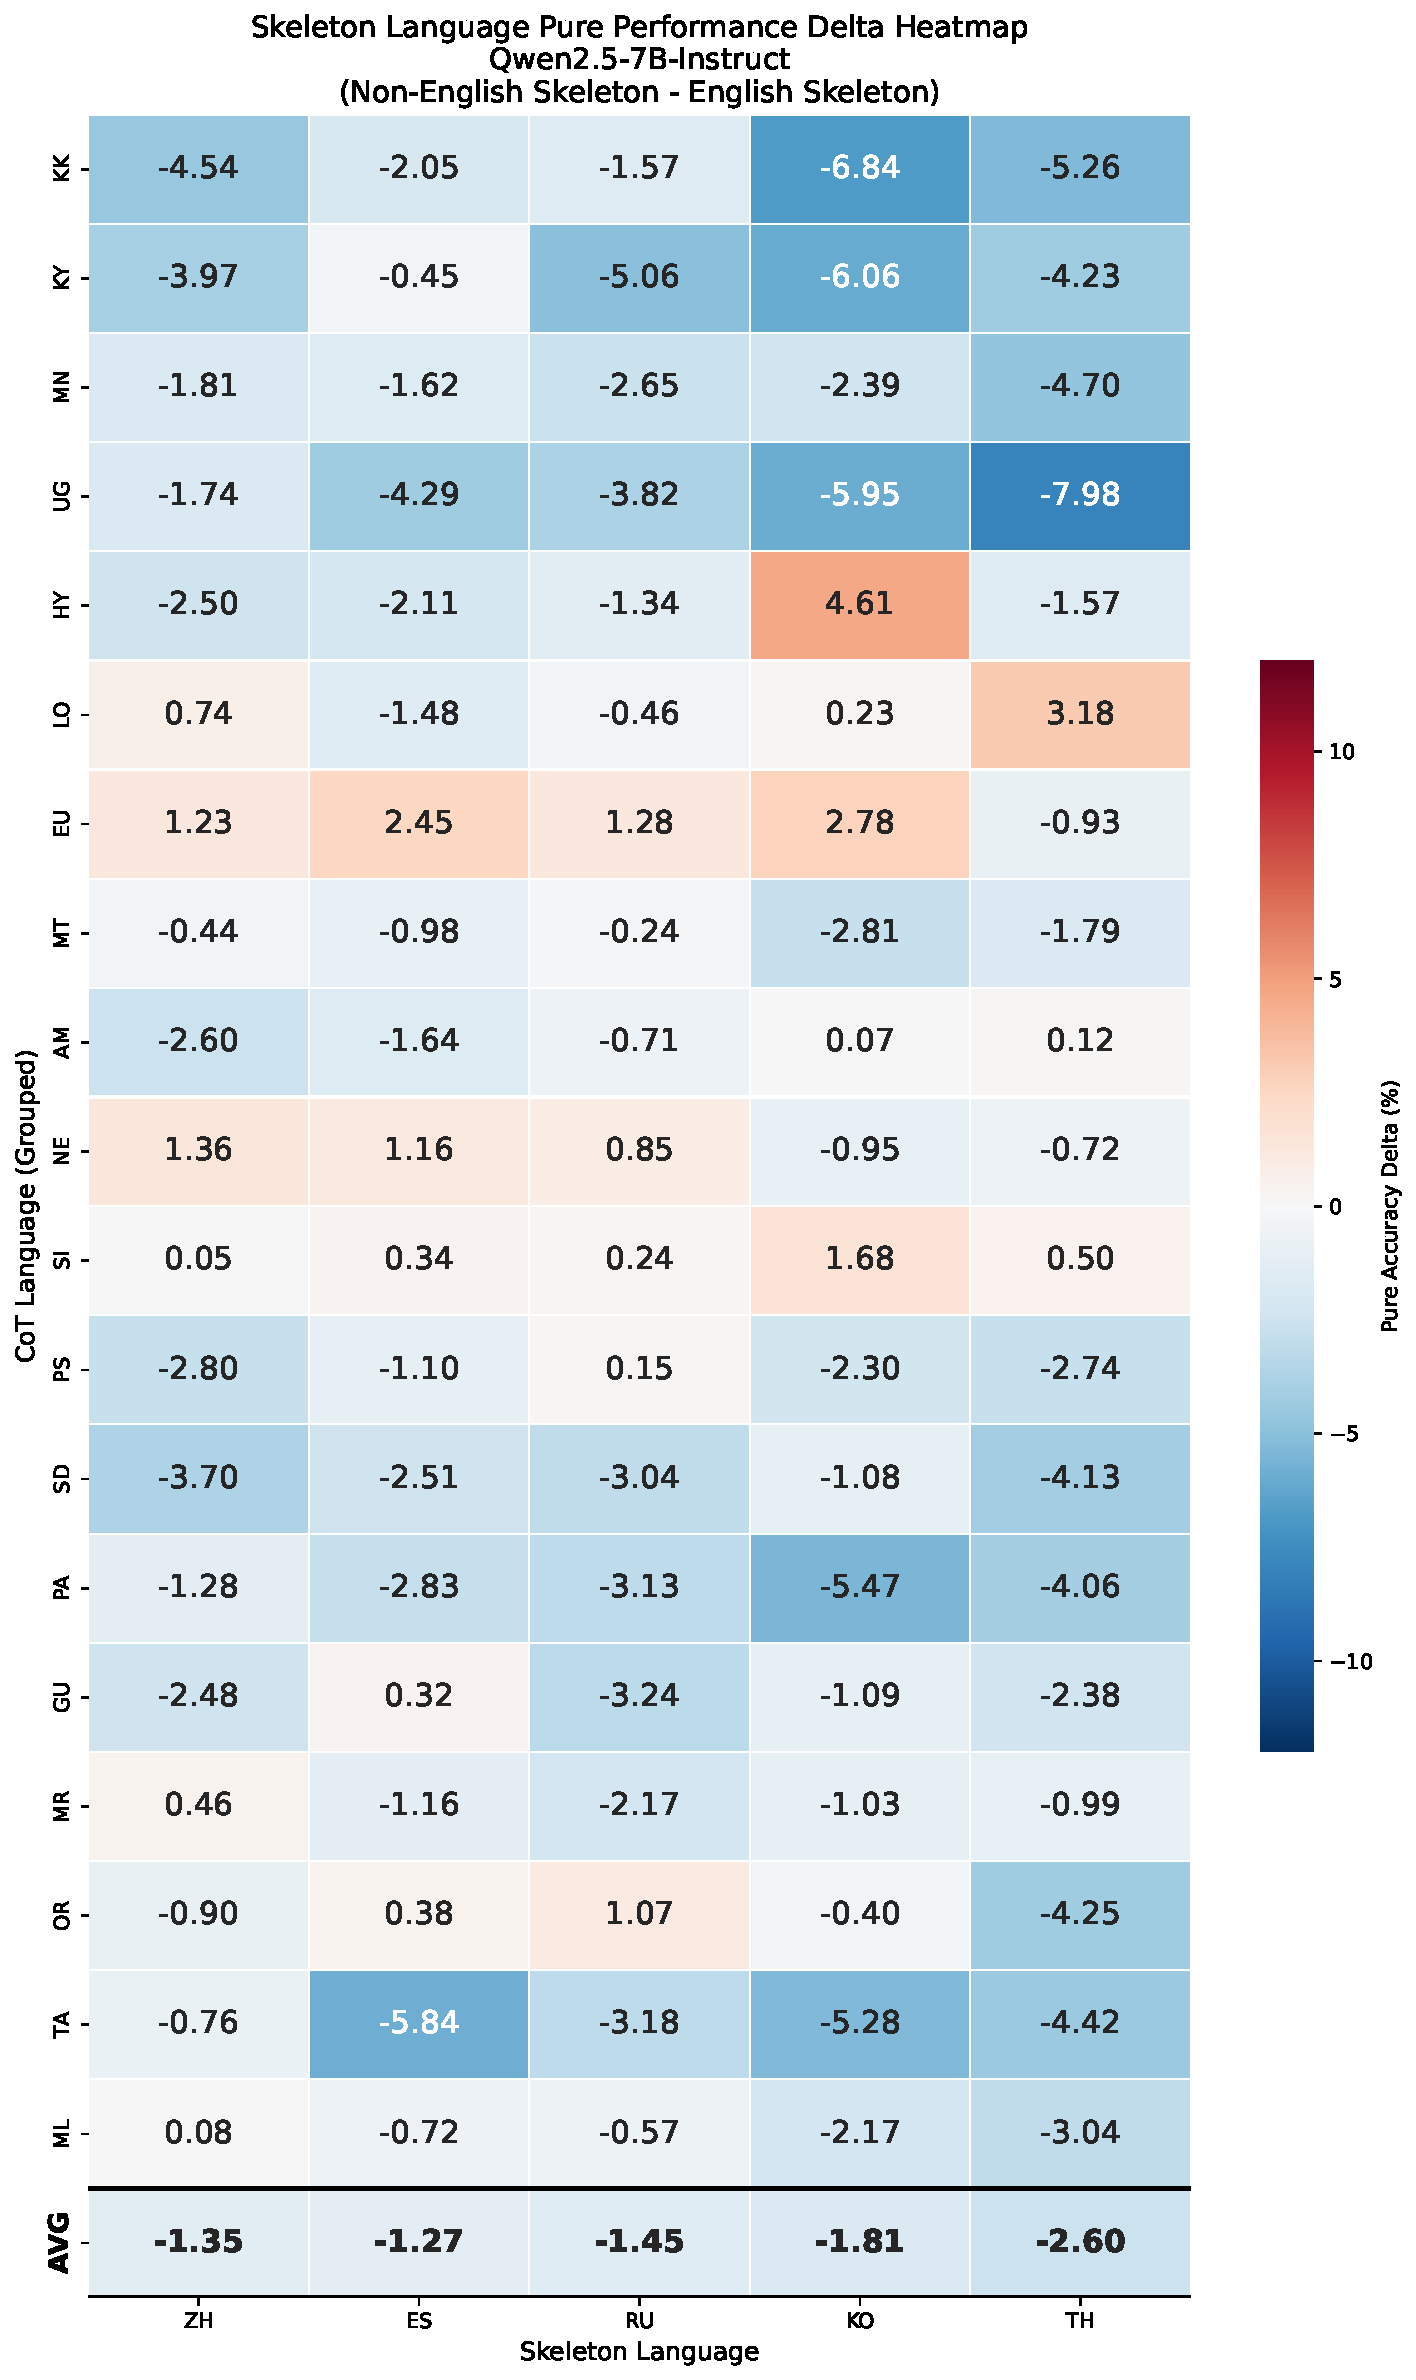
\includegraphics[width=\linewidth]{Figures/Images/Qwen2.5-7B-Instruct_rollout5_pure_delta_heatmap_sorted.pdf}
    \caption{\small Multi-rollout robustness of skeleton-language effects on MGSM under the CoT-$\ell_t$ setting with \textsc{Qwen2.5-7B}. Each cell reports the average performance difference (Non-English $-$ English) over five stochastic rollouts, where the English skeleton is replaced with one of five Non-English skeletons (ZH, ES, RU, KO, and TH). Compared with the single-rollout results in Figure~\ref{fig:cross-lingual-skeleton}, many apparent gains from Non-English skeletons are attenuated or reversed, suggesting that such gains are often sensitive to generation variability rather than consistently robust across rollouts.}
    \label{fig:cross-lingual-skeleton-rollout}
    \vspace{-0.15in}
\end{figure}